This work considers two well-known distributed localization protocols for testing the proposed localization procedure: Lateration and Bounding-Box. Some of their differences are highlighted in Table~\ref{table:protocols}.

\begin{table}[tb]
  \centering
  \begin{threeparttable}[t]
    \caption{Localization Protocols' characteristics}
    \label{table:protocols}
    \begin{tabular}{c||c||c}
    \hline
    \bfseries Characteristic & \bfseries Lateration & \bfseries Bounding-Box\\
    \hline\hline 
    Env. Conditions & At least 4 \emph{Anchors} & At least 1 \emph{Anchor}\\
    Accuracy & 2-10 meters & Coarse\tnote{1}\\
    Energy Consumption & Low~\cite{laterationSpecs} & Very low\tnote{2}\\
    \hline
    \end{tabular}
    \begin{tablenotes}
    \item [1] Location area upper-bounded by \emph{Anchor}'s radio range (R).
    \item [2] Can be treated as a discrete problem.
    \end{tablenotes}
  \end{threeparttable}
\end{table}

In order to reveal the impact of the proposed localization procedure in terms of battery consumption, number of located nodes and localization error; a thousand simulations are performed per \emph{Anchor} density (from 10\% up to 100\% at 10\% increments) using a customized extension of the SENSE network simulator~\cite{sense}. The hardware and Medium Access (MAC) layer parameters implemented are presented in Table~\ref{tab:MAC_param}. Two propagation models are used: free space and a time-invariant and symmetrical shadowing model (from here on: Free space and Shadowing models respectively). The characteristics of the testing plane are highlighted in Table~\ref{tab:testingPlanes}. Nodes are randomly and uniformly distributed over the testing plane (as in Figure~\ref{fig:topology}) and the position estimation is based only on the received location information from Beacons. This is done to evaluate different \emph{Anchor} densities against a single \emph{unknown} node (i.e. 100\% \emph{Anchor} density means 
that a determined node will receive Beacons from all its neighbors and use the received location information to estimate its position, regardless if the recipient is an \emph{Anchor}).

To contrast the behavior of the localization procedure against the individual execution of the proposed localization protocols, the deployment considerations are set accordingly with the capabilities of the protocols (large network lifetime and coarse accuracy). The PME deterministically selects the appropriate protocols as it is explained in Section~\ref{PME}.

%The deployment considerations are set to require coarse network lifetime and coarse accuracy, which can be achieved with the tested localization protocols detailed in Table~\ref{table:protocols}. Also, the PME deterministically selects the appropriate localization protocol based only on the satisfaction of each of their best-working environmental conditions.

Results are shown with 99\% confidence intervals.

\begin{table}[tb]
  \begin{threeparttable}[t]
    \caption{Hardware and CSMA/CA Parameters}
    \label{tab:MAC_param}
    \begin{tabular}{c||c||c}
    \hline
    \bfseries Component & \bfseries Parameter & \bfseries Value\\
    \hline\hline 
    \multirow{8}{*}{Hardware} & Data rate & $19.2$~kbps\\ %1
			      & TX power & $0$~dBm\\ %2
			      & Reception threshold & $-148$~dBm\\ %3
			      & Carrier sense threshold & $-148$~dBm\\ %4
			      & Power consumption in TX mode & $24.75$~mW\\ %5
			      & Power consumption in RX/idle mode & $13.5$~mW\\ %6
			      & Power consumption in sleep mode & $15~\mu\rm{W}$\\ %7
			      %& Length of data field & $29$~bytes\\ %8
    \hline
    \multirow{4}{*}{CSMA/CA} & Headers & $11$~bytes\\ %1
			      & Beacon size & $40$~bytes\\ %2
			      & Contention window & $128$\\ %3
			      & Slot time & $417~\mu\rm{s}$\\ %4
    \hline
%     \multirow{1}{*}{Upper layers} & Network and Localization header & $150$~bits\\ %1
%     \hline
    \end{tabular}
  \end{threeparttable}
\end{table}

% The upper layer header shown in Table~\ref{tab:MAC_param} represents the data size of the Beacon packet, composed of the \emph{Anchor}'s position and other simulator-related parameters.

\begin{table}[tb]
  \centering
  \begin{threeparttable}[t]
  \caption{Characteristics of the testing plane based on~\cite{convexEstimation,fieldDimmensions}}
  \label{tab:testingPlanes}
  \begin{tabular}{c||c}
  \hline
  \bfseries Characteristic & \bfseries Value\\
  \hline\hline
  Area & $100\times100$~m$^{2}$\\
  Surface & Flat\\
  Distribution of nodes & Uniformly random\\
  \hline
  \end{tabular}
  \end{threeparttable} 
\end{table}

Each time a node connects with a new \emph{Anchor} (effectively receives its Beacons), the PME decides which localization protocol to execute. In the proposed simulation (and following Table~\ref{table:protocols}) if more than three \emph{Anchors} are connected to the \emph{unknown} node, then the PME will execute Lateration, otherwise Bounding-Box is selected. Further connections will lead the PME to reevaluate the node's situation and sequentially execute the appropriate localization protocol. As for Lateration, this can go on until six \emph{Anchors} are connected. Beyond this number, the accuracy refinements are not as significant to justify the penalty in battery consumption~\cite{beaconLimits}.

\begin{figure}[tb]
  \centering
  \includegraphics[width=0.7\linewidth, angle = -90]{section4/figures/topology.eps}
  \caption{Example random deployment of nodes
  \label{fig:topology}}
\end{figure}

\subsection{The effect of the tested channel models on the number of connection to \emph{Anchors}}\label{channel_considerations}
In Figure~\ref{fig:channelAndBeacons}, it is appreciated how the different propagation models affect the reception of Beacon packets; which in this evaluation is the sole environmental condition considered by the PME.

\begin{figure}[tb]
  \centering
  \includegraphics[width=0.7\linewidth, angle = -90]{section4/figures/avgBeaconPerNode.eps}
  \caption{Average number of \emph{Anchors} connected to each node}
  \label{fig:channelAndBeacons}
\end{figure}

Nodes in the Shadowing model are prone to more collisions than those in the Free space model. When there is high concentration of neighboring \emph{Anchors}, it is more probable that collisions occur. This results in a decreased number of \emph{Anchors} connected to each node, which has a direct impact on battery life, accuracy and number of located nodes.

\subsection{Individual execution of Lateration and Bounding-Box localization protocols}\label{individual_execution}
In order to better analyze the impact of the localization procedure on the network, metrics are gathered from the individual execution of the tested localization protocols.

These metrics reflect the protocols' impact on battery consumption, number of located nodes and the position estimation error.

\subsubsection{Battery consumption}\label{individual_battery_consumption}
apart from the battery consumption related with the normal operation of the nodes (listening the channel and Beacon reception), Lateration has an additional battery consumption associated with the execution of the algorithm (as mentioned in Section~\ref{lateration}). This seems to be increased in the Free space model because of the greater average number of \emph{Anchors} connected to each node (see Figure~\ref{fig:channelAndBeacons}~and~\ref{fig:battery}).

\begin{figure}[tb]
  \centering
  \includegraphics[width=0.7\linewidth, angle = -90]{section4/figures/battery.eps}
  \caption{Battery consumption of the individual execution of Lateration and Bounding-Box
  \label{fig:battery}}
\end{figure}

In the case of Bounding-Box, there is not additional battery consumption related to the execution of this algorithm. This is the reason why its added battery consumption is considered negligible when compared to Lateration.

%As for Bounding-Box, the algorithm seems to impose almost none additional battery consumption on the nodes. It is considered negligible compared to that of Lateration.

\subsubsection{Located nodes}
these are the nodes that successfully execute either of the localization protocols, resulting in a location estimation (see Figure~\ref{fig:locNodes}).

\begin{figure}[tb]
  \centering
  \includegraphics[width=0.7\linewidth, angle = -90]{section4/figures/locatedNodes.eps}
  \caption{Number of located nodes per tested localization protocol
  \label{fig:locNodes}}
\end{figure}

In the case of Lateration, at 30\% \emph{Anchor} density around 84\% and 95\% of the nodes get located in the Free space and Shadowing models respectively. Lower numbers are appreciated at 10-20\% \emph{Anchor} density due to the reduced/inexistent Beacons received at these densities.

Bounding-Box shows higher number of located nodes at 30\% \emph{Anchor} density (nearly 99\% in both propagation models) mainly due to a more coarse restriction for the execution of this protocol (only one Beacon).

\subsubsection{Error}
the proposed measure of error only considers nodes that were able to execute either of the localization protocols. It is defined as the straight line distance (in meters) between the node's estimated location and its real position (see Figure~\ref{fig:error}).

\begin{figure}[tb]
  \centering
  \includegraphics[width=0.7\linewidth, angle = -90]{section4/figures/error.eps}
  \caption{Straight line error from the estimated to the real node's position
  \label{fig:error}}
\end{figure}

The error in Lateration is related to inexact ranging measurements, which is greater in the Shadowing model given that for the calculations the node always assumes a Free space model. The location accuracy does not seem to improve significantly with the connection of more than six \emph{Anchors} without sacrificing battery life~\cite{beaconLimits}. Furthermore, it worsens with the degraded channel conditions imposed by the Shadowing propagation model.

For Bounding-Box, the Shadowing model reduces the average number of \emph{Anchors} received at the \emph{unknown} node, which translates in the elimination of some of the constraints that allow this protocol to increase its accuracy.

%For Bounding Box, the Shadowing model shows that there are \emph{Anchors} at more than R (R = simulated radio range calculated in free space) meters from the \emph{unknown} node that are also considered in the calculation, thus increasing the size of the location area estimated by the algorithm. 

\subsection{Localization procedure execution}\label{locProc_executions}
As mentioned in Section~\ref{PME}, PME will pick a localization protocol that given the node's environmental conditions, could comply with the deployment considerations.

\subsubsection{Battery consumption}
the difference between the battery consumption associated with the proposed localization procedure and that of Lateration is very small. For this reason they are considered similar (see Figure~\ref{pme:battery}).

\begin{figure}[tb]
  \centering
  \includegraphics[width=0.7\linewidth, angle = -90]{section4/figures/pmeBat.eps}
  \caption{Localization procedure's associated battery consumption when compared with Lateration
  \label{pme:battery}}
\end{figure}

Bounding-Box adds negligible battery consumption (as mentioned in Section~\ref{individual_battery_consumption}), therefore it is not included in Figure~\ref{pme:battery}, which only attempts to compare the average battery consumption of the individual execution of Lateration and the amount consumed by the proposed localization procedure.

\subsubsection{Located nodes}\label{locProc_locatedNodes}
the sum of located nodes (either with Lateration or Bounding-Box) reaches 99\% at \emph{Anchor} densities around 30\% (see Figure~\ref{pme:locNodes}).

\begin{figure}[tb]
  \centering
  \includegraphics[width=0.7\linewidth, angle = -90]{section4/figures/pmeLocNodes.eps}
  \caption{Located nodes with the proposed localization procedure
  \label{pme:locNodes}}
\end{figure}

With Free space model 100\% localization is achieved at 20\% \emph{Anchor} density. On the other hand, in the Shadowing model 100\% localization is achieved at slightly higher densities, on average around 40\%.

The number of located nodes with the proposed localization procedure exceeds those of Lateration, in fact Figure~\ref{pme:locNodes} looks more like the curves of Bounding-Box in Figure~\ref{fig:locNodes}.

\subsubsection{Error}
This measure illustrates the average distance in meters between each node's estimated location and its real position. The prefix \emph{Loc. Proc.} in Figure~\ref{pme:error} highlights the fact that these are results gathered from the execution of the localization procedure.

\begin{figure}[tb]
  \centering
  \includegraphics[width=0.7\linewidth, angle = -90]{section4/figures/pmeAverageErrorPerProtocol.eps}
  \caption{Associated error after protocol selection
  \label{pme:error}}
\end{figure}

Figure~\ref{pme:error} displays the average error for each type of channel model. It also considers the number of nodes executing either Lateration or Bounding-Box. So the average error is expressed as: $Avg_{A}^{ch} = (E_{L}~n_{L} + E_{BB}~n_{BB}) /n_{L}+n_{BB}$. Where $Avg_{A}^{ch}$ is the average error with a $ch$ channel model and $A$ \emph{Anchor} density. $n_{L}$ are the number of nodes executing Lateration while $n_{BB}$ are the same but in the case of Bounding-Box. $E_{L}$ and $E_{BB}$ refer to the average line error for nodes executing Lateration and Bounding-Box respectively.

Due to increased ranging measurement errors, the estimation in the Shadowing model presents more erroneous estimations than the Free space model, as in Figure~\ref{fig:error}. Although at $30$\% \emph{Anchor} density the localization procedure incurs in greater average error as compared with the individual execution of Lateration, it manages to increase the average number of located nodes. This is significantly important, given that without the localization procedure many nodes were to be left without a location estimation, or what it is the same as having an undetermined measure of error.

A carefully selected set of localization protocols working with different ranges of environmental conditions, ensures that most of the nodes in the deployment get located. In the testings presented in this section, Bounding-Box is the responsible for locating the most isolated nodes, while Lateration focuses on accuracy. Selecting and characterizing more accurate protocols will reduce the errors and maintain the high number of located nodes that the localization procedure achieves. All of this while preserving the levels of battery consumption similar to the individual execution of the selected protocols.